
%TEMA 4

\section{La organización en Twitter, Inc.}

La función de organización se basa, principalmente, en dividir el trabajo, tanto humano como material, para posteriormente coordinar las distintas tareas de forma agrupada para la correcta ejecución de los planes establecidos. Para esta organización debemos tener en cuenta distintos factores, como la misión, los objetivos de la empresa, el uso de herramientas para la construcción de esta estructura, entre otros.

Twitter, Inc. mantiene, claramente, una estructura adhocratica, debido a su complejidad y a su dinamismo.

En la empresa que analizamos, Twitter, Inc., ya hemos mencionado anteriormente algunos de estos (como la misión).

\newpage

\subsection{Organigrama.}

\begin{figure}[!htb]
\centering
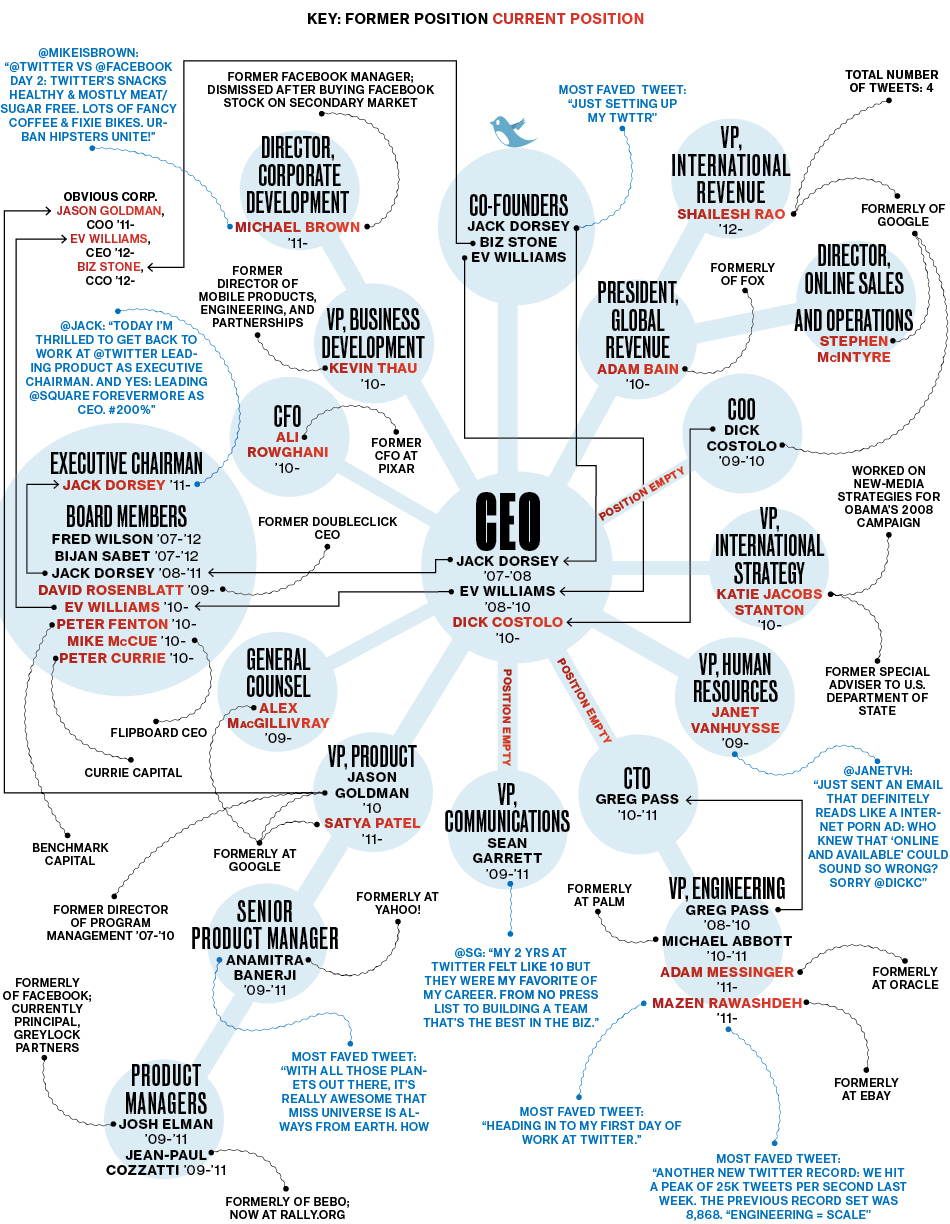
\includegraphics[scale=0.2]{organigrama.jpg}
\caption{\label{fig:frog}Organigrama Twitter, Inc. 2012}
\end{figure}


\subsection{Principios organizativos fundamentales.}

\subsubsection{Principio de la división del trabajo.}

Siguiendo estos principio, Twitter, Inc., se distribuye en distintos equipos de trabajo, entre los que se encuentran:\\

\textbf{Equipo Construir el producto}

El grupo \textit{Build the product} comprende los siguientes equipos:

\begin{itemize}

\item \textit{Data Science and Analytics}

Encargado de comprender como el mundo utiliza Twitter y como son sus usuarios.

\item \textit{Infraestructure Engineering}

Encargado de innovar, construir y mantener la infraestructura y servicios de Twitter operativos.

\item \textit{Product}

Encargado de desarrollar el producto principal, Twitter.

\item \textit{Software Engineering}

Encargado de desarrollar todos los servicios necesarios  en los que se basa Twitter, como por ejemplo Bootstrap.

\item \textit{User Services}

Encargado de dar soporte a los usuarios de Twitter siempre que lo necesiten.

\item \textit{Design and Research}

Encargados de mantener el diseño y características de Twitter a la última.

\end{itemize}

\textbf{Equipo Seguir manteniéndonos}

El grupo \textit{Keep us running} comprende los siguientes equipos:

\begin{itemize}

\item \textit{Finance}

Encargado de controlar las finanzas de Twitter, haciendo posible que sus productos sean rentables.

\item \textit{Legal and Public Policy}

Encargado de defender legalmente a la compañía y a sus usuario. 

\item \textit{People}

Encargado de los Recursos Humanos de Twitter, intentando que sea un lugar serio a la vez que agradable para trabajar.

\item \textit{Workplace}

Encargado de que las oficinas de Twitter sean lo más cómodas y útiles, para un correcto desarrollo de sus empleados.

\end{itemize}

\textbf{Equipo Promover el negocio}

El grupo \textit{Promote the business} comprende los siguientes equipos:

\begin{itemize}

\item \textit{Marketing and Communications}

Encargado de enseñar al mundo los avances realizados en Twitter.

\item \textit{Sales and Partnerships}

Encargado de trabajar en conjunto con otras marcas y compañías para alcanzar sus objetivos de forma conjunta y más sencilla.

\end{itemize}

\textbf{Equipo Nuestras marcas}

El grupo \textit{Our family of brands} comprende los siguientes equipos:

\begin{itemize}

\item \textit{Periscope}
\item \textit{MoPub}\\

\end{itemize}



Todos estos equipos se distribuyen entre más 35 países alrededor del mundo.

\subsubsection{Principio de la especialización del trabajo.}

Como vemos en el apartado anterior, existen grandes distinciones entre los distintos equipos de trabajo, por lo que es necesaria una especialización, que dependerá de cada equipo, encontrando así un alto nivel de especialización en cada uno de ellos.

\subsubsection{Principio de jerarquía, unidad de mando y ámbito de control.}

Estos principios, explicados y revisados en apartados anteriores, suponen una correcta organización del trabajo, esencial para el desarrollo de los objetivos de la empresa.

\subsubsection{Principio de descentralización.}

Como hemos visto, en Twitter, Inc. vemos una clara descentralización con los distintos grupos de trabajo, sin obviar las decisiones tomadas por los altos directivos.

\subsection{Adoctrinamiento y preparación de los empleados.}

Twitter, Inc. sigue un claro ejemplo de adoctrinamiento departamental, en el que prepara a sus empleados según el departamento al que pertenezcan, ya que, como hemos visto, su separación en equipos hace que esto sea más fácil de realizar.


\subsection{Factores de contingencia.}

\subsubsection{Entorno.}

En Twitter, Inc. encontramos un entorno dinámico, debido al constante cambio tecnológico, vemos una gran incertidumbre, lo que hace más difícil predecir cambios en el entorno, ademas, presenta un entorno complejo, ya que es necesario un alto nivel de formación, conocimiento, y habilidades para resolver los problemas planteados durante el desarrollo de la empresa.

\subsubsection{Edad.}

Twitter, Inc. fue fundada en 2006, esto hace que su organización no este aún muy consolidada, debido a la falta de madurez, aunque esto podría interpretarse como algo positivo, ya que permite adaptarse a la complejidad y dinamismo del entorno.

\subsubsection{Tamaño.}

En los últimos años, sobre todo desde 2012, Twitter, Inc., ha sufrido un fuerte crecimiento en su base de usuarios, lo que le ha permitido crecer de forma significativa su tamaño como empresa.

Actualmente, Twitter, Inc. cuenta con 336 millones de usuarios activos (datos del primer cuatrimestre de 2018) y con 3.372 empleados (2017).

\subsubsection{Tecnología.}

El principal desarrollo de Twitter, Inc. como empresa se basa en el desarrollo tecnológico, por lo que vemos que este tiene un gran impacto, tanto a nivel administrativo como económico dentro de la empresa, y esto lo podemos ver en la importancia de sus departamentos, la mayoría centrados en desarrollo de software, y en sus distintas tecnologías, usadas para apoyarse en el desarrollo de su aplicación principal, Twitter, como por ejemplo, Bootstrap, Gizzard Scala, FlockDB, entre otros.


\subsubsection{El entorno y la organización.}

En Twitter, Inc. encontramos un en entorno diversificado, ya que Twitter, Inc. se tiene que adaptar a distintos tipos de clientes, zonas geográficas, etc, para dar a conocer y expandir su producto. Ademas, el entorno es competitivo, ya que vemos como cada día surgen nuevas empresas competidoras, o ha de competir con otras con experiencia, como pueden ser Facebook, Instagram, Snapchat, etc, sumando el que al ser de tipo tecnológico, el alto nivel de incertidumbre impida reconocer posibles futuros competidores.

\subsection{La estructura de Twitter, Inc.}

Twitter, Inc. presenta claramente una estructura adhocrática, ya que, como hemos visto en el organigrama y en al analizar la dirección ejecutiva de la empresa, la parte más importante de Twitter, Inc. es el ápice estratégico y el núcleo operativo, pudiendo considerar este último como "doble", uno trabajando en los proyectos principales, como Twitter o Periscope, y el segundo núcleo de operaciones, que se alterara según sea necesario para la realización de otros proyectos, un ejemplo serian los ya mencionados como Bootstrap, Gizzard Scala o FlockDB.





%TEMA 5

\section{El entorno en Twitter, Inc.}
%TODO


%TEMA 6

\section{La dirección estratégica en Twitter, Inc.}

La estrategia representa la relación entre la empresa con su entorno y las acciones que emprende para realizar sus objetivos, haciendo un uso racional de sus recursos, con el objetivo de mejorar el rendimiento de la empresa.

El proceso de dirección estratégica consta de tres partes.

\subsection{Análisis estratégico.}

Se realiza un análisis de la misión y los objetivos de la empresa, junto con un análisis tanto externo como interno de esta (DAFO) y de los objetivos de propietarios y stakeholders.

\subsection{Formulación de estrategias.}

Una vez realizados los análisis previos, la empresa propone alternativas u opciones estratégicas  que deben ser consideradas tanto a nivel operativo, como a nivel funcional.

Twitter, Inc., en varias ocasiones ha formulado distintos tipos de estrategias.

\subsubsection{Estrategias competitivas.}

Para hacer frente a sus rivales, intentando remodelar sus productos, haciéndolos más atractivos y útiles de cara al público, como por ejemplo, la implementación de contenido personalizado a cada usuario, o el avance en la interacción de usuarios en su principal servicio, Twitter.

\subsubsection{Estrategias corporativas.}

Planteando la expansión de su negocio, con plataformas como Periscope, o MoPub, que han permitido a Twitter, Inc. crecer a nivel corporativo, y mantener la atención, tanto de competidores como de posibles stakeholders, gracias la diversidad de productos que le ha aportado estas estrategias corporativas.

\subsection{Implantación de la estrategia.}

Una vez formulada la estrategia, esta ha de implantarse en todos los niveles de la empresa, para cumplir con su objetivo, obtener una ventaja competitiva, algo que Twitter, Inc. consiguió con respecto a otras empresas del sector, lo que condujo a una mayor penetración en el mercado y el cumplimiento de su Misión y objetivos.


\section{La dirección de la producción y la innovación.}

Como todas las empresas, Twitter, Inc. busca una máxima producción con el menor costo posible, es decir, una gran productividad.

Actualmente, Twitter, Inc. se encuentra en el punto de crecimiento como empresa, ya que como veremos en el análisis financiero, tras muchos años de balance negativo, en el primer cuatrimestre de 2018 Twitter, Inc. llego a tener un balance positivo, generando ingresos y marcando lo que posiblemente sea el paso al crecimiento, que conduzca a la madurez de la empresa.

\subsection{Diseño del proceso productivo.}

Vemos como Twitter, Inc. , como todas las empresas tecnológicas, se centran en un proceso productivo de alto volumen, ya que pretenden que sus productos lleguen a un gran publico, y de alta variedad, para ser capaz de satisfacer a todo ese público, ademas de ser capaz de no depender de un único producto.

\subsection{Innovación.}

Gran parte de que Twitter, Inc. sea capaz de alcanzar sus objetivos, depende de la innovación, Twitter, Inc. ha de ser capaz de comercializar las ideas implantadas en sus productos, para que estos se expandan y tenga éxito.

\subsubsection{Tipo de innovación.}

Twitter, Inc. lleva a cabo una innovación tecnológica, ya que trabaja sobre un mercado existente, como son las Redes Sociales (principalmente), pero intentando implementar nuevas tecnologías y formas de comunicación.

\subsubsection{Investigación y Desarrollo.}

Normalmente, la investigación y desarrollo de las empresas forman parte del staff de apoyo de la empresa, ya que no formara parte del proceso productivo, y se limita a ayudar a la empresa, sin embargo, debido a la gran importancia del desarrollo tecnológico y la investigación, formara parte del proceso productivo de la empresa.

\subsubsection{Gestión de la innovación.}

Para Twitter, Inc. es tan importante la propiedad industrial, para mantener su imagen como marca y sus signos distintivos, como la propiedad intelectual, debido a la dependencia de trabajo tecnológico, que ha de ser protegido a través de derechos de autor.


\subsection{Alianzas para Twitter, Inc.}

En Twitter, Inc. , son muy importantes las alianzas horizontales complementarias, ya que, como empresa tecnológica, Twitter, Inc. no puede pretender hacerse cargo de todo lo necesario para almacenar, procesar y mostrar la información necesaria para sus productos, y un ejemplo de este tipo de alianzas son las alianzas realizadas con Google, o Amazon para almacenar datos en sus servidores, o las de otras empresas como Samsung, con las que se comprometieren a dar publicidad a cambio de incluir por defecto su software en sus dispositivos.

\subsection{Spin-Offs}

Tras el desarrollo de sus productos principales, Twitter, Inc. ha visto la posibilidad de creación de nuevos productos, que podrían generar grandes beneficios, un ejemplo de estos son Periscope y MoPub.

\subsubsection{Periscope.}

Tras el lanzamiento, y gran difusión de Twitter, una parte de la compañía Twitter, Inc vio la posibilidad de ampliar los servicios de su producto, llegando a un punto en el que se ideo un nuevo producto a partir del original, y así nació Periscope, como la idea de ampliar Twitter a un servicio de vídeo en streaming que fuera capaz de conectar a personas de todo el mundo, en cualquier momento.

\subsubsection{MoPub.}

Tras la primera etapa de Twitter, la publicidad en esta se convirtió en su principal fuente de ingresos, sin embargo, vieron que esto quedaba muy limitado al uso de Twitter, por lo que se creo MoPub, un servicio que procura dar visibilidad y monetizar los lanzamientos de desarrolladores de aplicaciones y servicios.